%\documentstyle[11pt,fullpage]{article}
%\setlength{\parindent}{0 in}
%\setlength{\parskip}{.1in}
%\setlength{\topmargin}{-0.5in}
%\setlength{\textheight}{8.5in}
%\begin{document}
\chapter{Mobile Networking in ns}
\label{chap:mobility}

This chapter describes the wireless model that was originally ported as CMU's Monarch group's mobility extension to \ns. 
This chapter consists of two sections and several subsections. The first section covers the original mobility model ported from CMU/Monarch group. In this section, we cover the internals of a mobilenode, routing mechanisms and network components that are 





















used to construct the network stack for a mobilenode. The components that are covered briefly are Channel, Network-interface, Radio propagation model, MAC protocols, Interface Queue, Link layer and Address resolution protocol model (ARP). CMU trace suppor





















t and Generation of node movement and traffic scenario files are also covered in this section.
The original CMU model allows simulation of pure wireless LANs or multihop ad-hoc networks. Further extensions were made to this model to allow combined simulation of wired and wireless networks. MobileIP was also extended to the wireless model. These are





















 discussed in the second section of this chapter.		


\section{The basic wireless model in ns}
\label{sec:basic-model}

The wireless model essentially consists of the MobileNode at the core,with
additional supporting features that allows simulations of multi-hop ad-hoc
networks, wireless LANs etc. The MobileNode object is a split object. The
C++ \clsref{MobileNode}{../ns-2/mobilenode.h} is derived from parent
\clsref{Node}{../ns-2/node.h}. Refer to Chapter~\ref{chap:nodes} for
details on \code{Node}. A \code{MobileNode} thus is the basic \code{Node}
object with added functionalities of a wireless and mobile node like
ability to move within a given topology, ability to receive and transmit
signals to and from a wireless channel etc. A major difference between
them, though, is that a \code{MobileNode} is not connected by means of
\code{Links} to other nodes or mobilenodes. In this section we shall
describe the internals of \code{MobileNode}, its routing mechanisms, the
routing protocols dsdv and dsr, creation of network stack allowing channel
access in \code{MobileNode}, brief description of each stack component,
trace support and movement/traffic scenario generation for wireless
simulations. 


\subsection{Mobilenode: creating wireless topology}
\label{sec:mobilenode-creation}

\code{MobileNode} is the basic \ns \code{Node} object with added
functionalities like movement, ability to transmit and receive on a
channel that allows it to be used to create mobile, wireless simulation
environments. The class MobileNode is derived from the base class Node.
\code{MobileNode} is a split object. The mobility features including node
movement, periodic position updates, maintaining topology boundary etc are
implemented in C++ while plumbing of network components within
\code{MobileNode} itself (like classifiers, dmux , LL, Mac, Channel etc)
have been implemented in Otcl. The functions and procedures described in
this subsection can be found in \nsf{mobilenode.\{cc,h\}},
\nsf{tcl/lib/ns-mobilenode.tcl}, \nsf{tcl/mobility/dsdv.tcl},
\nsf{tcl/mobility/dsr.tcl}. Example scripts can be found in
\nsf{tcl/ex/wireless-test.tcl} and \nsf{tcl/ex/wireless.tcl}. While the
first example uses a small topology of 3 nodes, the second example runs
over a topology of 50 nodes. These scripts can be run simply by typing

\begin{program}
$ns tcl/ex/wireless.tcl (or /wireless-test.tcl)
\end{program}

The two ad-hoc routing protocols that are currently supported are Destination Sequence Distance Vector (DSDV) and Dynamic Source Routing (DSR). The APIs for creating a mobilenode depends on which routing protocol it would be using. Hence the primitive to 





















create a mobilenode is

\begin{program}
	set mnode [$opt(rp)-create-mobile-node $id] 
\end{program}
where \$opt(rp) defines "dsdv" or "dsr" and id is the index for the mobilenode.

The above procedure creates a mobilenode (split)object, creates a routing agent as specified, creates the network stack consisting of a link layer, interface queue, mac layer, and a network interface with an antenna, interconnects these components and con





















nects the stack to the channel. The mobilenode now looks like the schematic in Figure~\ref{fig:mobilenode-dsdv}. 
\begin{figure}
    \centerline{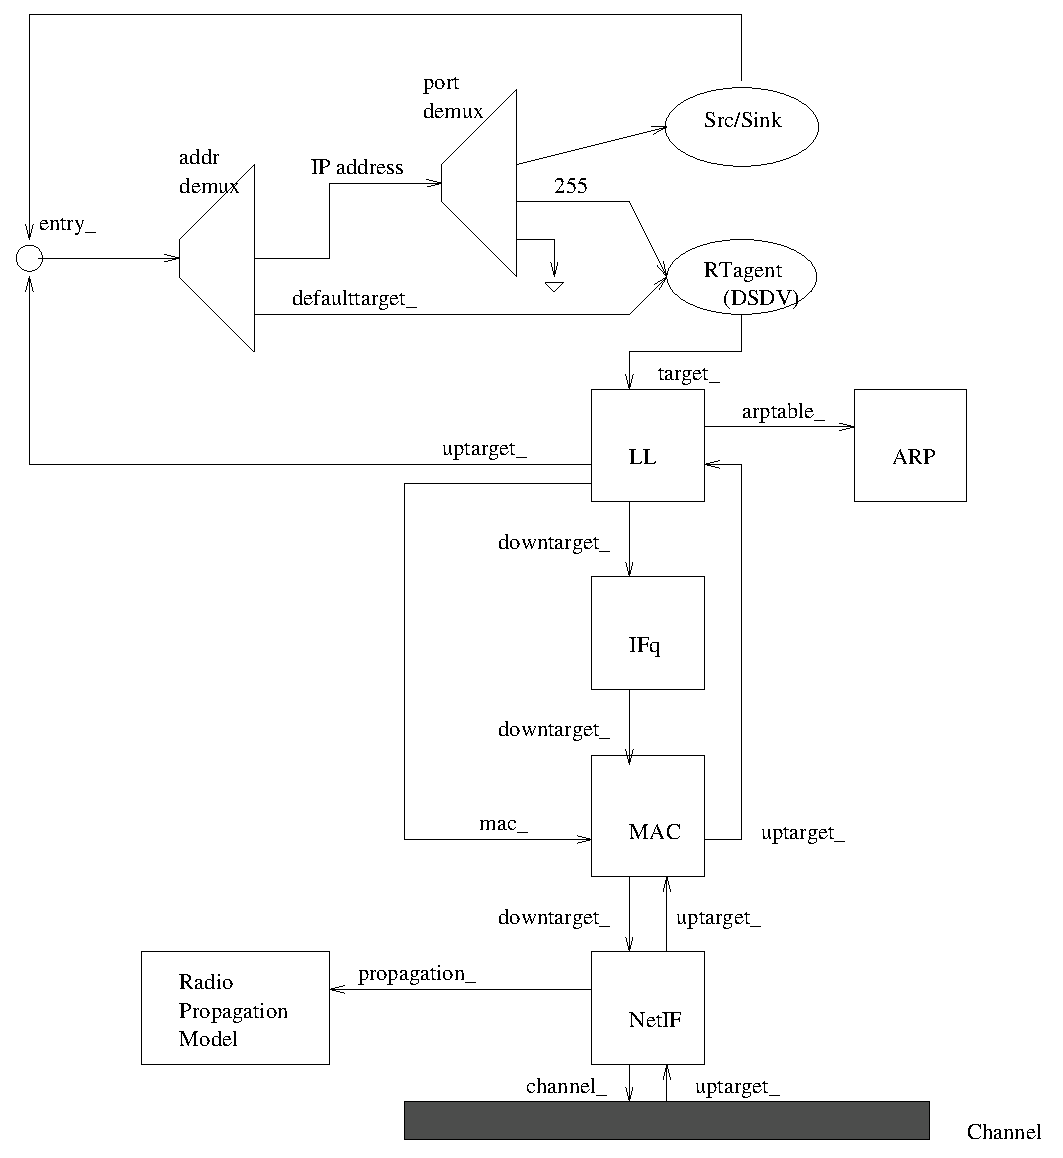
\includegraphics{dsdv}}
    \caption{Schematic of a mobilenode under the CMU monarch's wireless extensions to \ns}
    \label{fig:mobilenode-dsdv}
\end{figure}

The mobilenode structure used for DSR routing is a little different from the mobilenode described above. The class SRNode is derived from class MobileNode. SRNode doesnot use address demux or classifiers and all packets received by the node are handed dow





















n to the DSR routing agent by default. The DSR routing agent either receives pkts for itself by handing it over to the port dmux or forwards pkts as per source routes in the pkt hdr or sends out route requests and route replies for fresh packets. Details 





















on DSR routing agent may be found in section~\ref{sec:dsr}. The schematic model for a SRNode is shown in Figure~\ref{fig:mobilenode-dsr}.
\begin{figure}[tb]
    \centerline{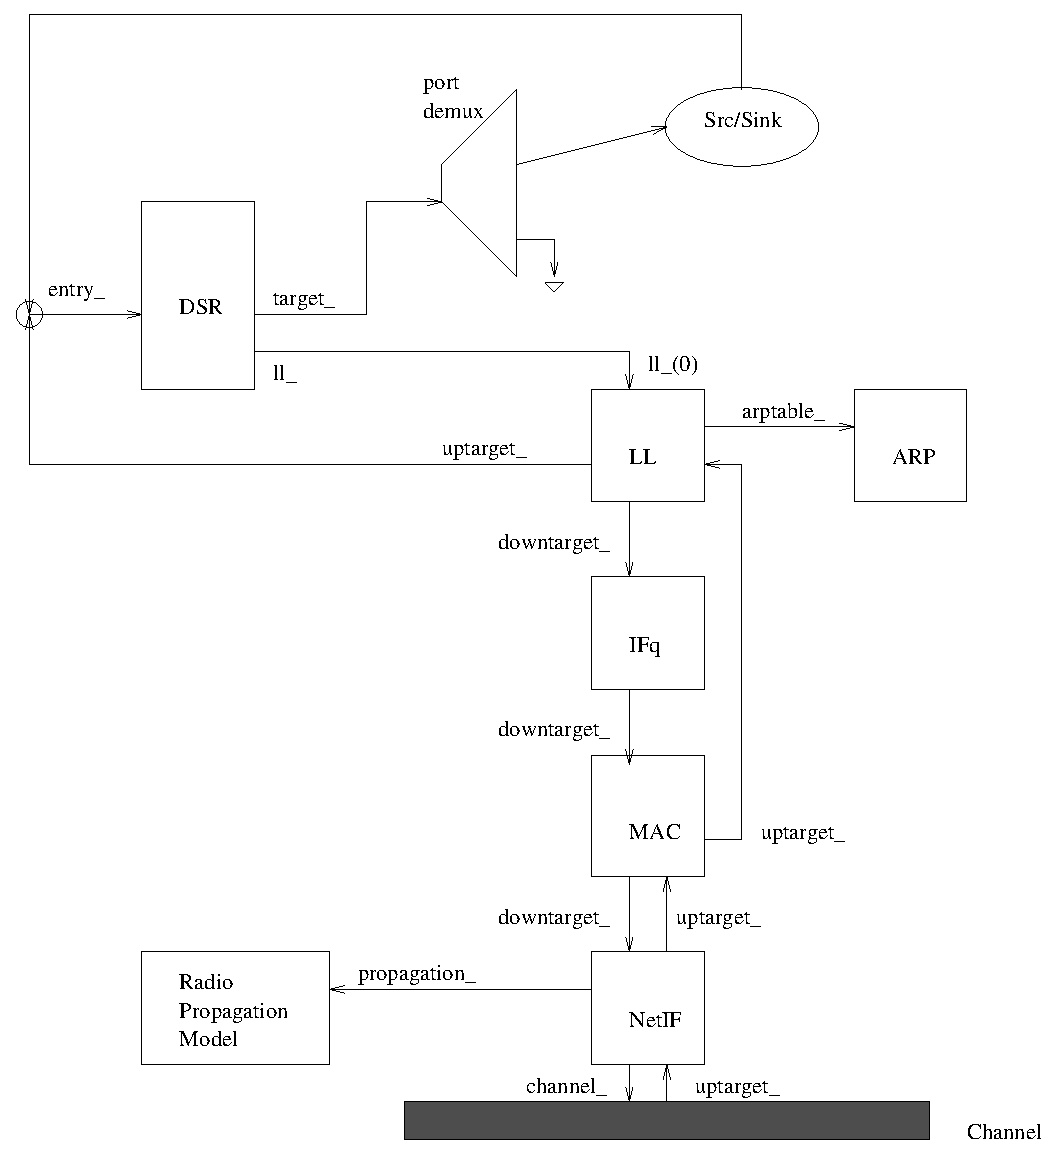
\includegraphics{dsr}}
    \caption{Schematic of a SRNode under the CMU monarch's wireless extensions to \ns}
    \label{fig:mobilenode-dsr}
\end{figure}

\subsection{Creating Node movements}
\label{sec:mobilenode-movements}

The mobilenode is designed to move in a three dimensional topology. However the third dimension (Z) is not used. That is the mobilenode is assumed to move always on a flat terrain with Z always equal to 0.
Thus the mobilenode has X, Y, Z(=0) co-ordinates that is continually adjusted as the node moves. There are two mechanisms to induce movement in mobilenodes. 
In the first method, starting position of the node and its future destinations may be set explicitly. These directives are normally included in a separate movement scenario file. 

The start-position and future destinations for a mobilenode may be set by using the following APIs:

\begin{program}

$node set X_ <x1>
$node set Y_ <y1>
$node set Z_ <z1>

$ns at $time $node setdest <x2> <y2> <speed>
\end{program}
At \$time sec, the node would start moving from its initial position 
of (x1,y1) towards a destination (x2,y2) at the defined speed.

In this method the node-movement-updates are triggered whenever the position of the node at a given time is required to be known. This may be triggered by a query from a neighbouring node seeking to know the distance between them, or the setdest directive





















 described above that changes the direction and speed of the node.

An example of a movement scenario file using the above APIs, can be found in \nsf{tcl/mobility/scene/scen-670x670-50-600-20-0}. Here 670x670 defines the length and width of the topology with 50 nodes moving at a maximum speed of 20m/s with average pause t





















ime of 600s. These node movement files may be generated using CMU's scenario generator to be found under ~ns/indep-utils/cmu-scen-gen/setdest.See subsection~\ref{sec:mobile-scen-generator} for details on generation of node movement scenarios.

The second method employs random movement of the node. The primitive to be used is:

\begin{program}
$mobilenode start
\end{program}
which starts the mobilenode with a random position and have routined updates to change the direction and speed of the node. The destination and speed values are generated in a random fashion. We have not used the second method and leave it to the user to 





















explore the details. 
The mobilenode movement is implemented in C++. See methods in ~ns/mobilenode.{cc.h} for the implementational details.

Irrespective of the methods used to generate node movement,
the topography for mobilenodes needs to be defined. It should be defined before creating mobilenodes. Normally flat topology is created by specifying the length and width of the topography using the following primitive:
\begin{program}	   
set topo	[new Topography]
$topo load_flatgrid $opt(x) $opt(y)
\end{program}
where opt(x) and opt(y) are the boundaries used in simulation.

The movement of mobilenodes may be logged by using a procedure like the following:

\begin{program}
proc log-movement \{\} \{
    global logtimer ns_ ns

    set ns $ns_
    source ../mobility/timer.tcl
    Class LogTimer -superclass Timer
    LogTimer instproc timeout \{\} \{
	global opt node_;
	for \{set i 0\} \{$i < $opt(nn)\} \{incr i\} \{
	    $node_($i) log-movement
	\}
	$self sched 0.1
    \}

    set logtimer [new LogTimer]
    $logtimer sched 0.1
\}
\end{program}
In this case, mobilenode positions would be logged every 0.1 sec.


\subsection{Network Components in a mobilenode}
\label{sec:mobilenode-components}

The network stack for a mobilenode consists of a link layer(LL), an ARP module connected to LL, an interface priority queue(IFq), a mac layer(MAC), a network interface(netIF), all connected to the channel. 
These network components are created and plumbed together in OTcl.
The relevant MobileNode method add-interface() in \nsf{tcl/lib/ns-mobilenode.tcl} is shown below:

\begin{program}
#
#  The following setups up link layer, mac layer, network interface
#  and physical layer structures for the mobile node.
#
Node/MobileNode instproc add-interface \{ channel pmodel 
		lltype mactype qtype qlen iftype anttype \} \{

	$self instvar arptable_ nifs_
	$self instvar netif_ mac_ ifq_ ll_

	global ns_ MacTrace opt

	set t $nifs_
	incr nifs_

	set netif_($t)	[new $iftype]		;# net-interface
	set mac_($t)	[new $mactype]		;# mac layer
	set ifq_($t)	[new $qtype]		;# interface queue
	set ll_($t)	[new $lltype]		;# link layer
        set ant_($t)    [new $anttype]

	#
	# Local Variables
	#
	set nullAgent_ [$ns_ set nullAgent_]
	set netif $netif_($t)
	set mac $mac_($t)
	set ifq $ifq_($t)
	set ll $ll_($t)

	#
	# Initialize ARP table only once.
	#
	if \{ $arptable_ == "" \} \{
            set arptable_ [new ARPTable $self $mac]
            set drpT [cmu-trace Drop "IFQ" $self]
            $arptable_ drop-target $drpT
        \}

	#
	# Link Layer
	#
	$ll arptable $arptable_
	$ll mac $mac
	$ll up-target [$self entry]
	$ll down-target $ifq

	#
	# Interface Queue
	#
	$ifq target $mac
	$ifq set qlim_ $qlen
	set drpT [cmu-trace Drop "IFQ" $self]
	$ifq drop-target $drpT

	#
	# Mac Layer
	#
	$mac netif $netif
	$mac up-target $ll
	$mac down-target $netif
	$mac nodes $opt(nn)

	#
	# Network Interface
	#
	$netif channel $channel
	$netif up-target $mac
	$netif propagation $pmodel	;# Propagation Model
	$netif node $self		;# Bind node <---> interface
	$netif antenna $ant_($t)        ;# attach antenna

	#
	# Physical Channel
	#
	$channel addif $netif           ;# add to list of interfaces

	# ============================================================
	# Setting up trace objects
	
	if \{ $MacTrace == "ON" \} \{
	    #
	    # Trace RTS/CTS/ACK Packets
	    #
	    set rcvT [cmu-trace Recv "MAC" $self]
	    $mac log-target $rcvT


	    #
	    # Trace Sent Packets
	    #
	    set sndT [cmu-trace Send "MAC" $self]
	    $sndT target [$mac sendtarget]
	    $mac sendtarget $sndT

	    #
	    # Trace Received Packets
	    #
	    set rcvT [cmu-trace Recv "MAC" $self]
	    $rcvT target [$mac recvtarget]
	    $mac recvtarget $rcvT

	    #
	    # Trace Dropped Packets
	    #
	    set drpT [cmu-trace Drop "MAC" $self]
	    $mac drop-target $drpT
	\} else \{
	    $mac log-target [$ns_ set nullAgent_]
	    $mac drop-target [$ns_ set nullAgent_]
	\}

	# ============================================================

	$self addif $netif
\}
\end{program}

The plumbing in the above method creates the network stack we see in Figure~\ref{fig:mobilenode-dsdv}.

Each component is briefly described here. Hopefully more detailed docuentation from CMU shall be available in the future.
\begin{description}
\item[{\bf Link Layer}] The \code{LL} used by mobilenode is same as described in Chapter~\ref{chap:lan}. The only difference being the link layer for mobilenode, has an ARP module connected to it which resolves all IP to hardware (Mac) address conversions





















. Normally for all outgoing (into the channel) packets, the packets are handed down to the \code{LL} by the Routing Agent. The \code{LL} hands down packets to the interface queue. For all incoming packets (out of the channel), the mac layer hands up packe





















ts to the \code{LL} which is then handed off at the \code{node_entry_} point. The \clsref{LL}{../ns-2/ll.h} is implemented in \nsf{ll.\{cc,h\}} and \nsf{tcl/lan/ns-ll.tcl}.

\item [{\bf ARP}] The Address Resolution Protocol (implemented in BSD style) module receives queries from Link layer. If ARP has the hardware address for destination, it writes it into the mac header of the packet. Otherwise it broadcasts an ARP query, an





















d caches the packet temporarily. For each unknown destination hardware address, there is a buffer for a single packet. Incase additional packets to the same destination is sent to ARP, the earlier buffered packet is dropped. Once the hardware address of a





















 packet"s next hop is known, the packet is inserted into the interface queue. The \clsref{ARPTable}{../ns-2/arp.h} is implemented in \nsf{arp.\{cc,h\}} and \nsf{tcl/lib/ns-mobilenode.tcl}.

\item[{\bf Interface Queue}] The \clsref{PriQueue}{../ns-2/priqueue.h} is implemented as a priority queue which gives priority to routing 
rotocol packets, inserting them at the head of the queue. It supports
running a filter over all packets in the queue and removes those with
a specified destination address. See \nsf{priqueue.\{cc,h\}} for 
interface queue implementation.

\item[{\bf Mac Layer}] The IEEE 802.11 distributed coordination 
function (DCF) Mac protocol has been implemented by CMU. It uses a 
RTS/CTS/DATA/ACK pattern for all unicast packets and simply sends out
 DATA for all broadcast packets. The implementation uses both 
physical and virtual carrier sense. The \clsref{Mac802\_11}{../ns-2/mac-802\_11.h} is implemented in \nsf{mac-802\_11.\{cc,h\}}.

\item[{\bf Tap Agents}] \code{Agents} that subclass themselves as \clsref{Tap}{../ns-2/mac.h} defined in mac.h can register themselves with the mac object using method installTap(). If the particular Mac protocol permits it, the tap will promiscuously be 





















given all packets received by the mac layer, before address filtering is done. See \nsf{mac.\{cc,h\}} for \clsref{Tap} implementation.

\item[{\bf Network Interfaces}] The Network Interphase layer serves as a hardware interface which is used by mobilenode to access the channel. The wireless shared media interface is implemented as \clsref{Phy/WirelessPhy}{../ns-2/wireless-phy.h}. This int





















erface subject to collisions and the radio propagation model receives packets transmitted by other node interfaces to the channel. The interface stamps each transmitted packet with the meta-data related to the transmitting interface like the transmission 





















power, wavelength etc. This meta-data in pkt header is used by the propagation model in receiving network interface to determine if the packet has minimum power to be received and/or captured and/or detected (carrier sense) by the receiving node. The mode





















l approximates the DSSS radio interface (Lucent WaveLan direct-sequence spread-spectrum). See \nsf{phy.\{cc.h\}} and \nsf{wireless-phy.\{cc,h\}} for network interface implementations.

\item[{\bf Radio Propagation Model}]  It uses Friss-space attenuation ($1/r^2$) at near distances and an approximation to Two ray Ground ($1/r^4$) at far distances. The approximation assumes specular reflection off a flat ground plane. See \nsf{tworaygrou





















nd.\{cc,h\}} for implementation.

\item[{\bf Antenna}] An omni-directional antenna having unity gain is used by mobilenodes. See \nsf{antenna.\{cc,h\}} for implementation details.
\end{description}

\subsection{Routing Agent in mobilenode}
\label{sec:mobilenode-routing}

Currently there are two different ad-hoc routing protocols implemented for mobile networking in \ns. We will first briefly discuss DSDV and then DSR. Again hopefully we will have some detailed documentation from CMU/Monarch group.

\subsubsection{DSDV}
\label{sec:dsdv}

In this routing protocol routing messages are exchanged between neighbouring mobilenodes (i.e mobilenodes that are within range of one another). Routing updates may be triggered or routine. Updates are triggered in case a routing information from one of t





















he neighbours forces a change in the routing table.
A packet for which the route to its destination is not known is cached while routing queries are sent out. The pkts are cached until route-replies are received from the destination. There is a maximum buffer size for caching the pkts waiting for routing i





















nformation beyond which pkts are dropped.

All packets destined for the mobilenode are routed directly by the address dmux to its port dmux. The port dmux hands the packets to the respective destination agents. A port number of 255 is used to attach routing agent in mobilenodes. The mobilenodes al





















so use a default-target in their classifier (or address demux). In the event a target is not found for the destination in the classifier (which happens when the destination of the packet is not the mobilenode itself), the pkts are handed to the default-ta





















rget which is the routing agent. The routing agent assigns the next hop for the packet and sends it down to the link layer.

The routing protocol is mainly implemented in C++. See \nsf{dsdv} directory and \nsf{tcl/mobility/dsdv.tc}l for all procedures related to DSDV protocol implementation.


\subsubsection{DSR}
\label{sec:dsr}

This section briefly describes the functionality of the dynamic source routing protocol. As mentioned earlier the \code{SRNode} is different from the \code{MobileNode}.  The \code{SRNode}'s \code{entry\_} points to the DSR routing agent, thus forcing all 





















packets received by the node to be handed down to the routing agent. This model is required for future implementation of piggy-backed routing information on data packets which otherwise would not flow through the routing agent.

The DSR agent checks every data packet for source-route information. It forwards the packet as per the routing information. Incase it doesnot find routing information in the packet, it provides the source route, if route is known, or caches the packet and





















 sends out route queries if route to destination is not known. Routing queries, always triggered by a data packet with no route to its destination, are initially broadcast to all neighbours. Route-replies are send back either by intermediate nodes or the 





















destination node, to the source, if it can find routing info for the destination in the route-query.  It hands over all packets destined to itself to the port dmux.
In \code{SRNode} the port number 255 points to a null agent since the packet has already been processed by the routing agent.

See \nsf{dsr} directory and \nsf{tcl/mobility/dsr.tcl} for implementation
of DSR protocol. 


\subsection{Trace Support}
\label{sec:mobile-trace}

The trace support for wireless simulations currently use cmu-trace
objects. In the future this shall be extended to merge with trace and
monitoring support available in ns, which would also include nam support
for wireless modules. For now we will explain briefly with cmu-trace
objects and how they may be used to trace packets for wireless scenarios. 

The cmu-trace objects are of three types - \code{CMUTrace/Drop},
\code{CMUTrace/Recv} and \code{CMUTrace/Send}. These are used for tracing
packets that are dropped, received and sent by agents, routers, mac layers
or interface queues in \ns. The methods and procedures used for
implementing wireless trace support can be found under
\nsf{trace.\{cc,h\}} and \nsf{tcl/lib/ns-cmutrace.tcl}.

A cmu-trace object may be created by the following API:

\begin{program}
set sndT [cmu-trace Send "RTR" $self]
\end{program}
which creates a trace object, sndT, of the type \code{CMUTrace/Send} for tracing all packets that are sent out in a router. The trace objects may be used to trace packets in MAC, agents (routing or others), routers or any other NsObject. 

The cmu-trace object \code{CMUTrace} is derived from the base class \code{Trace}. See Chapter~\ref{chap:trace} for details on class \code{Trace}. The class \code{CMUTrace} is defined as the following:

\begin{program}
class CMUTrace : public Trace \{
public:
	CMUTrace(const char *s, char t);
	void	recv(Packet *p, Handler *h);
	void	recv(Packet *p, const char* why);

private:
	int off_arp_;
	int off_mac_;
	int off_sr_;

	char	tracename[MAX_ID_LEN + 1];
        int     tracetype;
        MobileNode *node_;

        int initialized() \{ return node_ && 1; \}

	int	command(int argc, const char*const* argv);
	void	format(Packet *p, const char *why);

	void	format_mac(Packet *p, const char *why, int offset);
	void	format_ip(Packet *p, int offset);

	void	format_arp(Packet *p, int offset);
	void	format_dsr(Packet *p, int offset);
	void	format_msg(Packet *p, int offset);
	void	format_tcp(Packet *p, int offset);
	void	format_rtp(Packet *p, int offset);
\};
\end{program}

The type field (described in \code{Trace} class definition) is used to
differentiate among different types of traces. For cmu-trace this can be
{\bf s} for sending, {\bf r} for receiving or {\bf D} for dropping a
packet. A fourth type {\bf f} is used to denote forwarding of a packet
(When the node is not the originator of the packet). 
Similar to the method Trace::format(), the CMUTrace::format() defines and
dictates the trace file format. The method is shown below: 

\begin{program}
void CMUTrace::format(Packet* p, const char *why)
\{
	hdr_cmn *ch = HDR_CMN(p);
	int offset = 0;

	/*
	 * Log the MAC Header
	 */
	format_mac(p, why, offset);
	offset = strlen(wrk_);

	switch(ch->ptype()) \{

	case PT_MAC:
		break;

	case PT_ARP:
		format_arp(p, offset);
		break;

	default:
		format_ip(p, offset);
		offset = strlen(wrk_);

		switch(ch->ptype()) \{

		case PT_DSR:
			format_dsr(p, offset);
			break;

		case PT_MESSAGE:
		case PT_UDP:
			format_msg(p, offset);
			break;
			
		case PT_TCP:
		case PT_ACK:
			format_tcp(p, offset);
			break;
			
		case PT_CBR:
			format_rtp(p, offset);
			break;
		..........

		\}
	\}
\}
\end{program}
The above function calls different format functions depending on the type
of the packet being traced. All traces are written to the buffer wrk\_. A
count of the offset for the buffer is kept and is passed along the
different trace functions. The most basic format is defined by
format\_mac() and is used to trace all pkt types. The other format
functions print additional information as defined by the packet types. The
mac format prints the following:   

\begin{program}
\#ifdef LOG_POSITION
        double x = 0.0, y = 0.0, z = 0.0;
        node_->getLoc(&x, &y, &z);
\#endif

	sprintf(wrk_ + offset,
\#ifdef LOG_POSITION
		"%c %.9f %d (%6.2f %6.2f) %3s %4s %d %s %d [%x %x %x %x] ",
\#else
		"%c %.9f _%d_ %3s %4s %d %s %d [%x %x %x %x] ",
\#endif
		op,                    // s, r, D or f
		Scheduler::instance().clock(),  // time stamp
                src_,                  // the nodeid for this node
\#ifdef LOG_POSITION
                x,                     // x co-ord 
                y,                     // y co-ord
\#endif
		tracename,             // name of object type tracing
		why,                   // reason, if any

                ch->uid(),             // identifier for this event
		packet_info.name(ch->ptype()), // packet type
		ch->size(),                    // size of cmn header
		mh->dh_duration,       // expected time to send data 
		ETHER_ADDR(mh->dh_da), // mac_destination address
		ETHER_ADDR(mh->dh_sa),         // mac_sender address
		GET_ETHER_TYPE(mh->dh_body));  // type - arp or IP
\end{program}

If the LOG\_POSITION is defined the x and y co-ordinates for the
mobilenode is also printed. The descriptions for different fields in the
mac trace are given in the comments above. For all IP packets additional
IP header fields are also added to the above trace. The IP trace is
described below:

\begin{program}
sprintf(wrk_ + offset, "------- [%d:%d %d:%d %d %d] ",
		src,          // IP src address
		ih->sport_,   // src port number
		dst,          // IP dest address
		ih->dport_,   // dest port number
		ih->ttl_,     // TTL value 
		(ch->next_hop_ < 0) ? 0 : ch->next_hop_); // next hopaddress, if any.
\end{program}

An example of a trace for a tcp packet is as follows:
\begin{program}
r 160.093884945 _6_ RTR  --- 5 tcp 1492 [a2 4 6 800] ------- [655
36:0 16777984:0 31 16777984] [1 0] 2 0
\end{program}
Here we see a TCP data packet being received by a node with id of 6. UID
of this pkt is 5 with a cmn hdr size of 1492. The mac details shows an IP
pkt (ETHERTYPE\_IP is defined as 0x0800, ETHERTYPE\_IP is 0x0806 ), mac-id
of this receiving node is 6. That of the sending node is 4 and expected
time to send this data pkt over the wireless channel is a2 (hex2dec
conversion: 160+2 sec). Additionally, IP traces information about IP src
and destination addresses. The src translates (using a 3 level
hier-address of 8/8/8) to a address string of 0.1.0 with port of 0. The
dest address is 1.0.3 with port address of 0. The TTL value is 31 and the
destination was a hop away from the src. Additionally TCP format prints
information about tcp seqno of 1, ackno of 0. See other formats described
in \nsf/cmu-trace.cc for DSR, UDP/MESSAGE, TCP/ACK and CBR packet types.

Other trace formats are also used by the routing agents (DSDV and DSR) to
log certain special events like "originating" (adding a SR header to a
packet) or  "ran off the end of a source route" indicating some sort of
routing problem with the source route etc. These special event traces may
be found in \nsf{dsdv/dsdv.cc} for DSDV and \nsf{dsr/dsrgent.cc} for DSR
routing agent.


\subsection{Revised format for wireless traces}
\label{sec:revtraceformat}

In an effort to merge wireless trace, using cmu-trace objects, with
ns tracing, a new, inproved trace format has been introduced. This revised
trace support is backwards compatible with the old trace formatting and
can be enabled by the following command:
\begin{program}
$ns use-newtrace
\end{program}
This command should be called before the universal trace command \code{$ns
trace-all <trace-fd>}. Primitive \code{use-newtrace} sets up new
format for wireless tracing by setting a simulator variable called
\code{newTraceFormat}. Currently this new trace support is available for
wireless simulations only and shall be extended to rest of \ns in the near
future.

An example of the new trace format is shown below:
\begin{program}
s -t 0.267662078 -Hs 0 -Hd -1 -Ni 0 -Nx 5.00 -Ny 2.00 -Nz 0.00 -Ne
-1.000000 -Nl RTR -Nw --- -Ma 0 -Md 0 -Ms 0 -Mt 0 -Is 0.255 -Id -1.255 -It
message -Il 32 -If 0 -Ii 0 -Iv 32
s -t 1.511681090 -Hs 1 -Hd -1 -Ni 1 -Nx 390.00 -Ny 385.00 -Nz 0.00 -Ne
-1.000000 -Nl RTR -Nw --- -Ma 0 -Md 0 -Ms 0 -Mt 0 -Is 1.255 -Id -1.255 -It
message -Il 32 -If 0 -Ii 1 -Iv 32
s -t 10.000000000 -Hs 0 -Hd -2 -Ni 0 -Nx 5.00 -Ny 2.00 -Nz 0.00 -Ne
-1.000000 -Nl AGT -Nw --- -Ma 0 -Md 0 -Ms 0 -Mt 0 -Is 0.0 -Id 1.0 -It tcp -Il 1000 -If
2 -Ii 2 -Iv 32 -Pn tcp -Ps 0 -Pa 0 -Pf 0 -Po 0
r -t 10.000000000 -Hs 0 -Hd -2 -Ni 0 -Nx 5.00 -Ny 2.00 -Nz 0.00 -Ne
-1.000000 -Nl RTR -Nw --- -Ma 0 -Md 0 -Ms 0 -Mt 0 -Is 0.0 -Id 1.0 -It tcp -Il 1000 -If
2 -Ii 2 -Iv 32 -Pn tcp -Ps 0 -Pa 0 -Pf 0 -Po 0
r -t 100.004776054 -Hs 1 -Hd 1 -Ni 1 -Nx 25.05 -Ny 20.05 -Nz 0.00 -Ne
-1.000000 -Nl AGT -Nw --- -Ma a2 -Md 1 -Ms 0 -Mt 800 -Is 0.0 -Id 1.0 -It
tcp -Il 1020 -If 2 -Ii 21 -Iv 32 -Pn tcp -Ps 0 -Pa 0 -Pf 1 -Po 0
s -t 100.004776054 -Hs 1 -Hd -2 -Ni 1 -Nx 25.05 -Ny 20.05 -Nz 0.00 -Ne
-1.000000 -Nl AGT -Nw --- -Ma 0 -Md 0 -Ms 0 -Mt 0 -Is 1.0 -Id 0.0 -It ack -Il 40
-If 2 -Ii 22 -Iv 32 -Pn tcp -Ps 0 -Pa 0 -Pf 0 -Po 0 
\end{program}

\subsubsection{Explanation of new trace format}
The new trace format as seen above can be can be divided into the
following fields :
\begin{description}
\item[Event type]
In the traces above, the first field (as in the older trace format)
describes the type of event taking place at the node and can be one of the 
four types:
\begin{description}
\item[s] send 
\item[r] receive 
]item[d] drop 
\item[f] forward
\end{description}

\item[General tag]
The second field starting with "-t" may stand for time or global setting
(****** explanation required)
\begin{description}
\item[-t] time
\item[-t] * (global setting)
\end{description}

\item[Node property tags]
This field denotes the node properties like node-id, the level at
which tracing is being done like agent, router or MAC. The tags start
with a leading "-N" and are listed as below:
\begin{description}
\item[-Ni:] node id
\item[-Nx:] node's x-coordinate
\item[-Ny:] node's y-coordinate
\item[-Nz:] node's z-coordinate
\item[-Ne:] node energy level
\item[-Nl:] trace level, such as AGT, RTR, MAC
\item[-Nw:] reason for the event. The different reasons for dropping a
packet are given below:
\begin{description}
\item["END"] DROP\_END\_OF\_SIMULATION          
\item["COL"] DROP\_MAC\_COLLISION              
\item["DUP"] DROP\_MAC\_DUPLICATE 
\item["ERR"] DROP\_MAC\_PACKET\_ERROR  
\item["RET"] DROP\_MAC\_RETRY\_COUNT\_EXCEEDED
\item["STA"] DROP\_MAC\_INVALID\_STATE      
\item["BSY"] DROP\_MAC\_BUSY                 

\item["NRTE"] DROP\_RTR\_NO\_ROUTE i.e no route is available.
\item["LOOP"] DROP\_RTR\_ROUTE\_LOOP i.e there is a routing loop
\item["TTL"]  DROP\_RTR\_TTL i.e TTL has reached zero.
\item["TOUT"] DROP\_RTR\_QTIMEOUT i.e packet has expired.
\item["CBK"]  DROP\_RTR\_MAC\_CALLBACK

\item["IFQ"]  DROP\_IFQ\_QFULL i.e no buffer space in IFQ.
\item["ARP"]  DROP\_IFQ\_ARP\_FULL i.e dropped by ARP
\item["OUT"]  DROP\_OUTSIDE\_SUBNET i.e dropped by base stations on
receiving routing updates from nodes outside its domain.
\end{description}
\end{description}

\item[Packet information at IP level]
The tags for this field start with a leading "-I" and are listed along
with their explanations as following:
\begin{description}
\item[-Is:] source address.source port number
\item[-Id:] dest address.dest port number
\item[-It:] packet type
\item[-Il:] packet size
\item[-If:] flow id
\item[-Ii:] unique id
\item[-Iv:] ttl value  
\end{description}

\item[Next hop info]
This field provides next hop info and the tag starts with a leading "-H".
\begin{description}
\item[-Hs:] id for this node
\item[-Hd:] id for next hop towards the destination.
\end{description}

\item[Packet info at MAC level]
This field gives MAC layer information and starts with a leading "-M" as
shown below:
\begin{description}
\item[-Ma:] duration
\item[-Md:] dst's ethernet address
\item[-Ms:] src's ethernet address
\item[-Mt:] ethernet type  
\end{description}     

\item[Packet info at "Application level"]
The packet information at application level consists of the type of
application like ARP, TCP, the type of adhoc routing protocol like
DSDV, DSR, AODV etc being traced. This field consists of a leading "-P"
and list of tags for different application is listed as below:
\begin{description}
\item[-P arp] Address Resolution Protocol. Details for ARP is given by the
following tags:
\begin{description}
\item[-Po:] ARP Request/Reply
\item[-Pm:] src mac address
\item[-Ps:] src address
\item[-Pa:] dst mac address
\item[-Pd:] dst address
\end{description}

\item[-P dsr] This denotes the adhoc routing protocol called Dynamic
source routing. Information on DSR is represented by the following tags:
\begin{description}
\item[-Pn:] how many nodes traversed
\item[-Pq:] routing request flag
\item[-Pi:] route request sequence number
\item[-Pp:] routing reply flag
\item[-Pl:] reply length
\item[-Pe:] src of srcrouting->dst of the source routing
\item[-Pw:] error report flag ?
\item[-Pm:] number of errors
\item[-Pc:] report to whom
\item[-Pb:] link error from linka->linkb
\end{description}

\item[-P cbr] Constant bit rate. Information about the CBR application is
represented by the following tags:

\begin{description}
\item[-Pi:] sequence number
\item[-Pf:] how many times this pkt was forwarded
\item[-Po:] optimal number of forwards 
\end{description}

\item[-P tcp] Information about TCP flow is given by the following
subtags:

\begin{description}
\item[-Ps:] seq number
\item[-Pa:] ack number
\item[-Pf:] how many times this pkt was forwarded
\item[-Po:] optimal number of forwards 
\end{description}
\end{description}

This field is still under development and new tags shall be added for
other applications as they get included along the way.
\end{description}


\subsection{Generation of node-movement and traffic-connection for wireless scenarios}
\label{sec:mobile-scen-generator}

Normally for large topologies, the node movement and traffic connection
patterns are defined in separate files for convinience. These movement and
traffic files may be generated using CMU's movement- and
connection-generators. In this section we shall describe both separately.

\subsubsection{MobileNode Movement}
\label{sec:mobile-movement-file}

Some examples of node movement files may be found in
\nsf{tcl/mobility/scene/scen-670x670-50-600-20-\{0,1,2\}. These files
define a topology of 670 by 670m where 50 nodes move with a speed of 20m/s
with pause time of 600s. each node is assigned a starting position. The
information regarding number of hops between the nodes is fed to the
central object "GOD" (XXX but why/where is this information used??-answer
awaited from CMU.) Next each node is a speed and a direction to move to. 

The generator for creating node movement files are to be found under \nsf{indep-utils/cmu-scen-gen/setdest/} directory. Compile the files under setdest to create an executable. run setdest with arguments in the following way:
\begin{program}
./setdest -n <num_of_nodes> -p <pausetime> -s <maxspeed> -t <simtime> -x <maxx> -y <maxy> > <outdir>/<scenario-file>
\end{program}
Note that the index used for nodes now start from 0 instead of 1 as was in the original CMU version, to match with \ns's tradition of assigning node indices from 0. 


\subsubsection{Generating traffic pattern files}
\label{sec:mobile-traffic-file}

The examples for traffic patterns may be found in \nsf{tcl/mobility/scene/cbr-50-\{10-4-512, 20-4-512\}}. 

The traffic generator is located under \nsf{indep-utils/cmu-scen-gen/} and are called cbrgen.tcl and tcpgen.tcl. They may be used for generating CBR and TCP connections respectively.

To create CBR connecions, run
\begin{program}
ns cbrgen.tcl [-type cbr|tcp] [-nn nodes] [-seed seed] [-mc connections] [-rate rate]
\end{program}
To create TCP connections, run
\begin{program}
ns tcpgen.tcl [-nn nodes] [-seed seed]
\end{program}
You will need to pipe the outputs from above to a cbr-* or a tcp-* file.



\section{Extensions made to CMU's wireless model}
\label{sec:wireless-extensions}

As mentioned earlier, the original CMU wireless model allows simulation of wireless LANs and ad-hoc networks. However in order to use the wireless model for simulations using both wired and wireless nodes we had to add certain extensions to cmu model. We 





















call this wired-cum-wireless feature. Also SUN's MobileIP (implemented for wired nodes) was integrated into the wireless model allowing mobileIP to run over wireless mobilenodes. The following two subsections describe these two extensions to the wireless 





















model in \ns. 


\subsection{wired-cum-wireless scenarios}
\label{sec:wired-cum-wireless}

The mobilenodes described so far mainly supports simulation of multi-hop ad-hoc networks or wireless LANs. But what if we need to simulate a topology of multiple wireless LANs connected through wired nodes, or may need to run mobileIP on top of these wire





















less nodes? The extensions made to the CMU wireless model allows us to do that.

The main problem facing the wired-cum-wireless scenario was the issue of routing. In ns, routing information is generated based on the connectivity of the topology, i.e how nodes are connected to one another through \code{Links}. Mobilenodes on the other 





















hand have no concept of links. They route packets among themselves, within the wireless topology, using their routing protocol. so how would packets be exchanged between these two types of nodes?
So a node called \code{BaseStationNode} is created which plays the role of a gateway for the wired and wireless domains. The \code{BaseStationNode} is essentially a hybrid between a Hierarchical node\footnote{Refer to Chapter~\ref{chap:hier-rtg} for detai





















ls on hierarchical routing and internals of \code{HierNode}.} (\code{HierNode}) and a \code{MobileNode}. The basestation node is responsible for delivering packets into and out of the wireless domain. In order to achieve this we need Hierarchical routing.





















 Each wireless domain along with its base-station would have an unique domain address assigned to them. All packets destined to a wireless node would reach the base-station attached to the domain of that wireless node, who would eventually hand the packet





















 over to the destination (mobilenode). And mobilenodes route packets, destined to outside their (wireless) domain, to their base-station node. The base-station knows how to forward these packets towards the (wired) destination. 
\begin{figure}
    \centerline{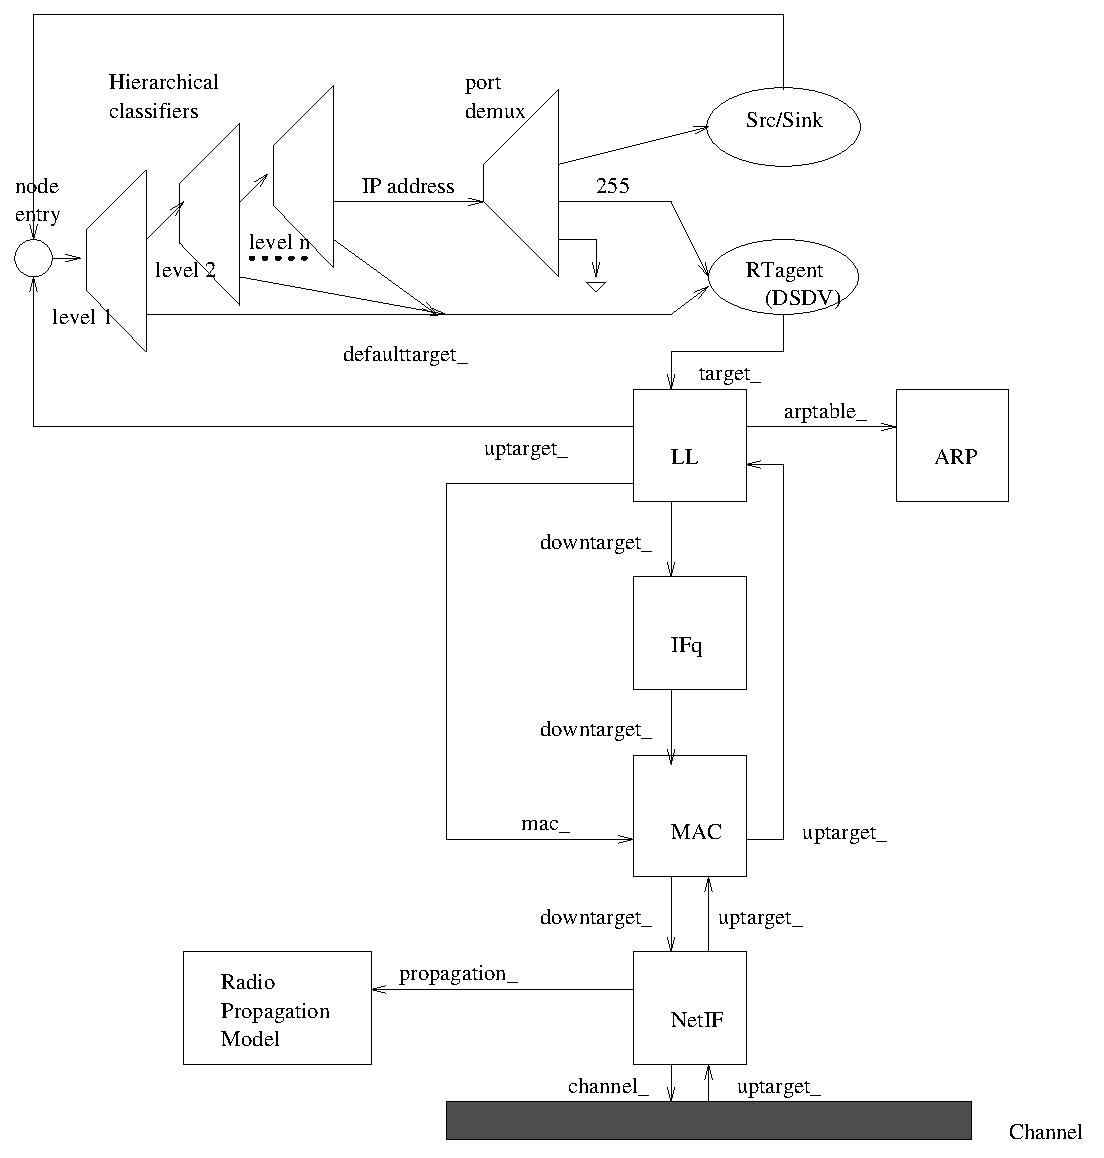
\includegraphics{basestation}}
    \caption{Schematic of a baseStationNode}
    \label{fig:mobilenode-basestation}
\end{figure}
The schematic of a \code{BaseStationNode} is shown in Figure~\ref{fig:mobilenode-basestation}.

The mobilenodes in wired-cum-wireless scenario are required to support hierarchical addressing/routing. Thus the \code{MobileNode} looks exactly like the \code{BaseStationNode}. The SRNode, however, simply needs to have its own hier-address since it doesn





















ot require any address demuxes and thus is not required to support hier routing\footnote{In order to do away with all these different variations of the definition of a node, we are planning to revise the node architecture that would allow a more flexible 





















and modularised construction of a node without the necessity of having to define and be limited to certain Class definitions only.}.

The DSDV agent on having to forward a packet checks to see if the destination is outside its (wireless) subnet. If so, it tries to forward the packet to its base-station node. In case no route to base-station is found the packet is dropped. Otherwise the 





















packet is forwarded to the next\_hop towards the base-station. Which is then routed towards the wired network by base-station's classifiers.

The DSR agent, on receiving a pkt destined outside its subnet, sends out a route-query for its base-station in case the route to base-station is not known. The data pkt is temporarily cached while it waits to hear route replies from base-station. On getti





















ng a reply the packet is provided with routing information in its header and send away towards the base-station. The base-station address demuxes routes it correctly toward the wired network. 

The example script for a wired-cum-wireless simulation can be found at \nsf{tcl/ex/wired-cum-wireless-sim.tcl}. The methods for wired-cum-wireless implementations are defined in \nsf{tcl/lib/ns-bsnode.tcl}, \nsf{tcl/mobility/\{com.tcl,dsr.tcl, dsdv.tcl\}}





















, \nsf{dsdv/dsdv.\{cc,h\}} and \nsf{dsr/dsragent.\{cc,h\}}.


\subsection{MobileIP}
\label{sec:mobileip}

The wired-cum-wireless extensions for the wireless model paved the path for supporting wireless MobileIP in \ns. Sun Microsystem's (Charlie Perkins etal) MobileIP model was based on ns's wired model (consisting of \code{Node}'s and \code{Link}'s) and thus





















 didnot use CMU's mobility model.

Here we briefly describe the wireless MobileIP implementation. We hope that Sun would provide the detailed version of the documentation in the future.

The mobileIP scenario consists of Home-Agents(HA) and Foreign-Agents(FA) and have Mobile-Hosts(MH) moving between their HA and FAs.
The HA and FA are essentially base-station nodes we have described earlier. While MHs are basically the mobileNodes described in section~\ref{sec:mobilenode-creation}.
The methods and procedures for MobileIP extensions are described in \nsf{mip.\{cc,h\}}, \nsf{mip-reg.cc}, \nsf{tcl/lib/ns-mip.tcl} and \nsf{tcl/lib/ns-wireless-mip.tcl}.

\begin{figure}
    \centerline{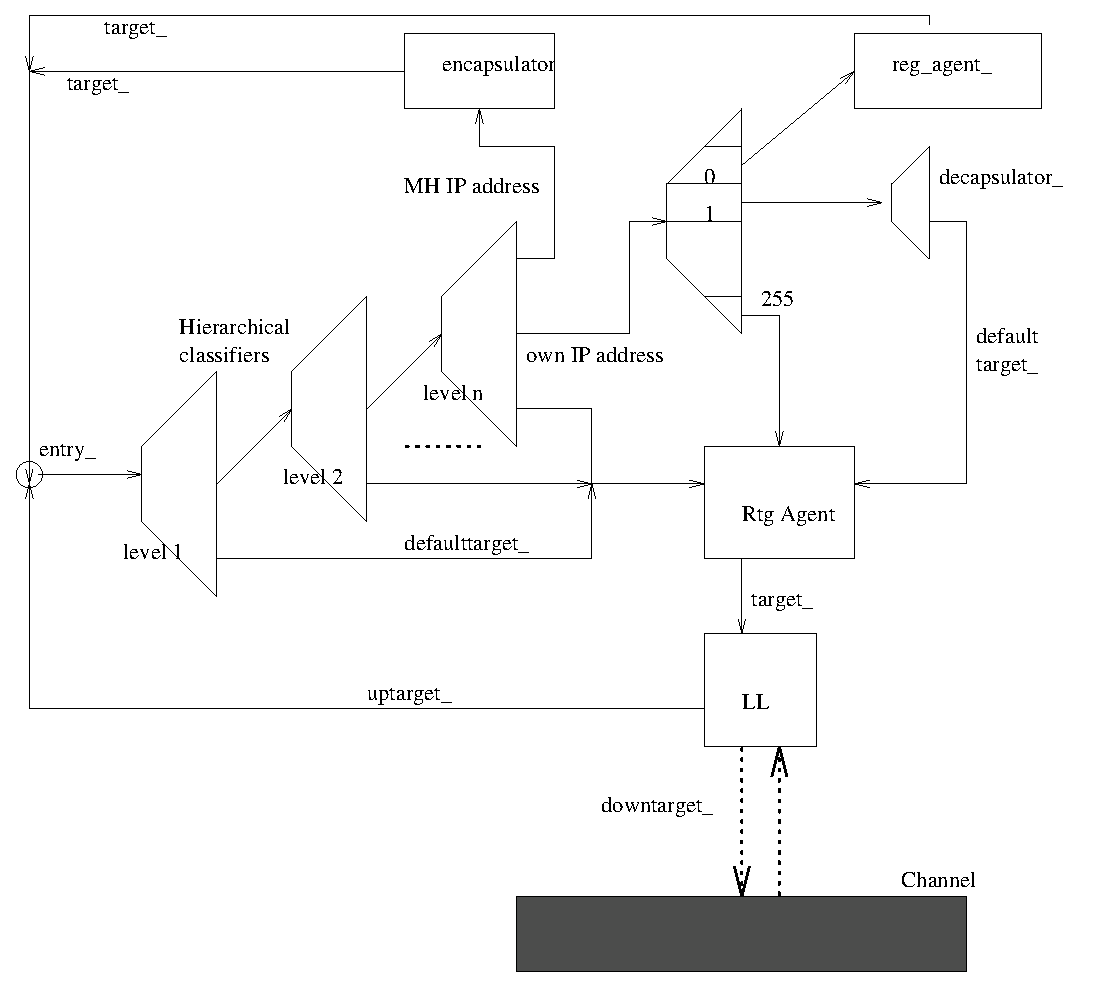
\includegraphics{wireless-mip}}
    \caption{Schematic of a Wireless MobileIP BaseStation Node}
    \label{fig:mobilenode-wireless-mip}
\end{figure}
The HA and FA nodes are defined as \code{MobileNode/MIPBS} having a registering agent (regagent\_) that sends beacon out to the mobilenodes, sets up encapsulator and decapsulator, as required and replies to solicitations from MHs. 
The MH nodes are defined as \code{MobileNode/MIPMH} which too have a regagent\_ that receives and responds to beacons and sends out solicitations to HA or FAs. Figure~\ref{fig:mobilenode-wireless-mip} illustrates the schematic of a \code{MobileNode/MIPBS}





















 node. The \code{MobileNode/MIPMH} node is very similar to this except for the fact that it doesnot have any encapsulator or decapsulator. As for the SRNode version of a MH, it doesnot have the hierarchical classifiers and the RA agent forms the entry poi





















nt of the node. See Figure~\ref{fig:mobilenode-dsr} for model of a SRNode.

The \code{MobileNode/MIPBS} node routinely broadcasts beacon or advertisement messages out to MHs. A solicitation from a mobilenode generates an ad that is send directly to the requesting MH. The address of the base-station sending out beacon is heard by 





















MH and is used as the COA (care-of-address) of the MH. Thus as the MH moves from its native to foreign domains, its COA changes.
Upon receiving  reg\_request (as reply to ads) from a mobilehost the base-station checks to see if it is the HA for the MH. If not, it sets up its decapsulator and forwards the reg\_request towards the HA of the MH. 
Incase the base-station {\em is} the HA for the requesting MH but the COA doesnot match its own, it sets up an encapsulator and sends reg-request-reply back to the COA (address of the FA) who has forwarded the reg\_request to it. so now all packets destin





















ed to the MH reaching the HA would be tunneled through the encapsulator which encapsulates the IP pkthdr with a IPinIP hdr, now destined to the COA instead of MH. The FA's decapsulator recives this packet, removes the encapsulation and sends it to the MH.






















If the COA matches that of the HA, it just removes the encapsulator it might have set up (when its mobilehost was roaming into foreign networks) and sends the reply directly back to the MH, as the MH have now returned to its native domain.

The mobilehost sends out solicitations if it doesnot hear any ads from the
base-stations. Upon receiving ads, it changes its COA to the address of
the HA/FA it has heard the ad from, and replies back to the COA with a
request for registration (\code{reg-request}).
Initially the MH maybe in the range of the HA and receives all pkts
directly from its COA which is HA in this case. 
Eventually as the MH moves out of range of its HA and into the a foreign
domain of a FA, the MH's COA changes from its HA to that of the FA. The HA
now sets up an encapsulator and tunnels all pkts destined for MH towards
the FA. The FA decapsulates the pkts and hands them over to the MH. The
data from MH destined for the wired world is always routed towards its
current COA.  
An example script for wireless mobileIP can be found at
\nsf{tcl/ex/wireless-mip-test.tcl}. The simulation consists of a MH moving
between its HA and a FA. The HA and FA are each connected to a wired
domain on one side and to their wireless domains on the other. TCP flows
are set up between the MH and a wired node. 


\section{Commands at a glance}
\label{sec:wirelesscommand}

Following is a list of commands used in wireless simulations:
\begin{program}
$ns_ node-config -addressingType <usually flat or hierarchical used for 
                                   wireless topologies>
                 -adhocRouting   <adhoc rotuing protocol like DSDV, DSR,
                                   TORA, AODV etc>
                 -llType         <LinkLayer>
                 -macType        <MAC type like Mac/802_11>
                 -propType       <Propagation model like
                                   Propagation/TwoRayGround>
                 -ifqType        <interface queue type like
                                   Queue/DropTail/PriQueue>
                 -ifqLen         <interface queue length like 50>
                 -phyType        <network inteface type like
                                   Phy/WirelessPhy>
                 -antType        <antenna type like Antenna/OmniAntenna>
                 -channelType    <Channel type like Channel/WirelessChannel>
                 -topoInstance   <the topography instance>
                 -wiredRouting   <turning wired routing ON or OFF>
                 -mobileIP       <setting the flag for mobileIP ON or OFF>
                 -energyModel    <EnergyModel type>
                 -initialEnergy  <specified in Joules>
                 -rxPower        <specified in W>
                 -txPower        <specified in W>
                 -agentTrace     <tracing at agent level turned ON or OFF>
                 -routerTrace    <tracing at router level turned ON or OFF>
                 -macTrace       <tracing at mac level turned ON or OFF>
                 -movementTrace  <mobilenode movement logging turned
                                   ON or OFF>
\end{program}
This command is used typically to configure for a mobilenode. For more info
about this command (part of new node APIs) see chapter titled "Restructuring
ns node and new Node APIs" in ns Notes and Documentation.

\begin{flushleft}
\code{$ns_ node <optional:hier address>}\\
This command is used to create a mobilenode after node configuration is done
as shown in the node-config command. Incase hierarchical addressing is being
used, the hier address of the node needs to be passed as well.


\code{$node log-movement}\\
This command previously used to enable logging of mobilenode's movement has now
been replaced by \code{$ns_ node-config -movementTrace <ON or OFF>}.


\code{create-god <num_nodes>}\\
This command is used to create a God instance. The number of mobilenodes
is passed as argument which is used by God to create a matrix to store
connectivity information of the topology.


\code{$topo load_flatgrid <X> <Y> <optional:res>}\\
This initializes the grid for the topography object. <X> and <Y> are the x-y
co-ordinates for the topology and are used for sizing the grid. The grid
resolution may be passed as <res>. A default value of 1 is normally used.


\code{$topo load_demfile <file-descrptor>}\\
For loading DEMFile objects into topography. See \ns/dem.{cc,.h} for details on
DEMFiles.


\code{$ns_ namtrace-all-wireless <namtrace> <X> <Y>}\\
This command is used to initialize a namtrace file for logging node movements
to be viewed in nam. The namtrace file descriptor, the X and Y 
co-ordinates of the wireless topology is passed as parameters with this command.


\code{$ns_ nam-end-wireless <stop-time>}\\
This command is used to tell nam the simulation stop time given by <stop-time>.


\code{$ns_ initial_node_pos <node> <size>}\\
This command defines the node initial position in nam. <size> denotes the size
of node in nam. This function must be called after mobility model has been
defined.


\code{$mobilenode random-motion <0 or 1>}\\
Random-motion is used to turn on random movements for the mobilenode, in which
case random destinations are assigned to the node. 0 disables and 1 enables
random-motion.


\code{$mobilenode setdest <X> <Y> <s>}\\
This command is used to setup a destination for the mobilenode. The mobile
node starts moving towards destination given by <X> and <Y> at a speed of
<s> m/s.


\code{$mobilenode reset}\\
This command is used to reset all the objects in the nodes (network 
components like LL, MAC, phy etc).


Internal procedures\\
Following is a list of internal procedures used in wireless networking:

\code{$mobilenode base-station <BSnode-hier-addr>}\\
This is used for wired-cum-wireless scenarios. Here the mobilenode is provided
with the base-stationnode info for its domain. The address is hierarchical
since wired-cum-wireless scenarios typically use hierarchical addressing.


\code{$mobilenode log-target  <target-object>}\\
The <target-object>, which is normally a trace object, is used to log
mobilenode movements and their energy usage, if energy model is provided.


\code{$mobilenode topography <topoinstance>}\\
This command is used to provide the node with a handle to the topography
object.


\code{$mobilenode addif}\\
A mobilenode may have more than one network interface. This command is used
to pass handle for a network interface to the node.


\code{$mobilenode  namattach <namtracefd>}\\
This command is used to attach the namtrace file descriptor <namtracefd>
to the mobilenode. All nam traces for the node are then written into this
namtrace file.


\code{$mobilenode radius <r>}\\
The radius <r> denotes the node's range. All mobilenodes that fall within
the circle of radius <r> with the node at its center are considered as
neighbours. This info is typically used by the gridkeeper.


\code{$mobilenode start}\\
This command is used to start off the movement of the mobilenode.

\end{flushleft}

%\end{document}
\endinput


